\documentclass[a4paper,landscape]{article}

\usepackage[landscape,top=0cm,left=0cm,bottom=0cm,right=0cm]{geometry}
\usepackage{tikz}
\usepackage{background}
\usepackage{blindtext}
\usetikzlibrary{matrix, shapes.misc, calc}

\pagestyle{empty}
\setlength{\parindent}{0cm}
\backgroundsetup{scale = 1, angle = 0, opacity = 1, color=black, contents = {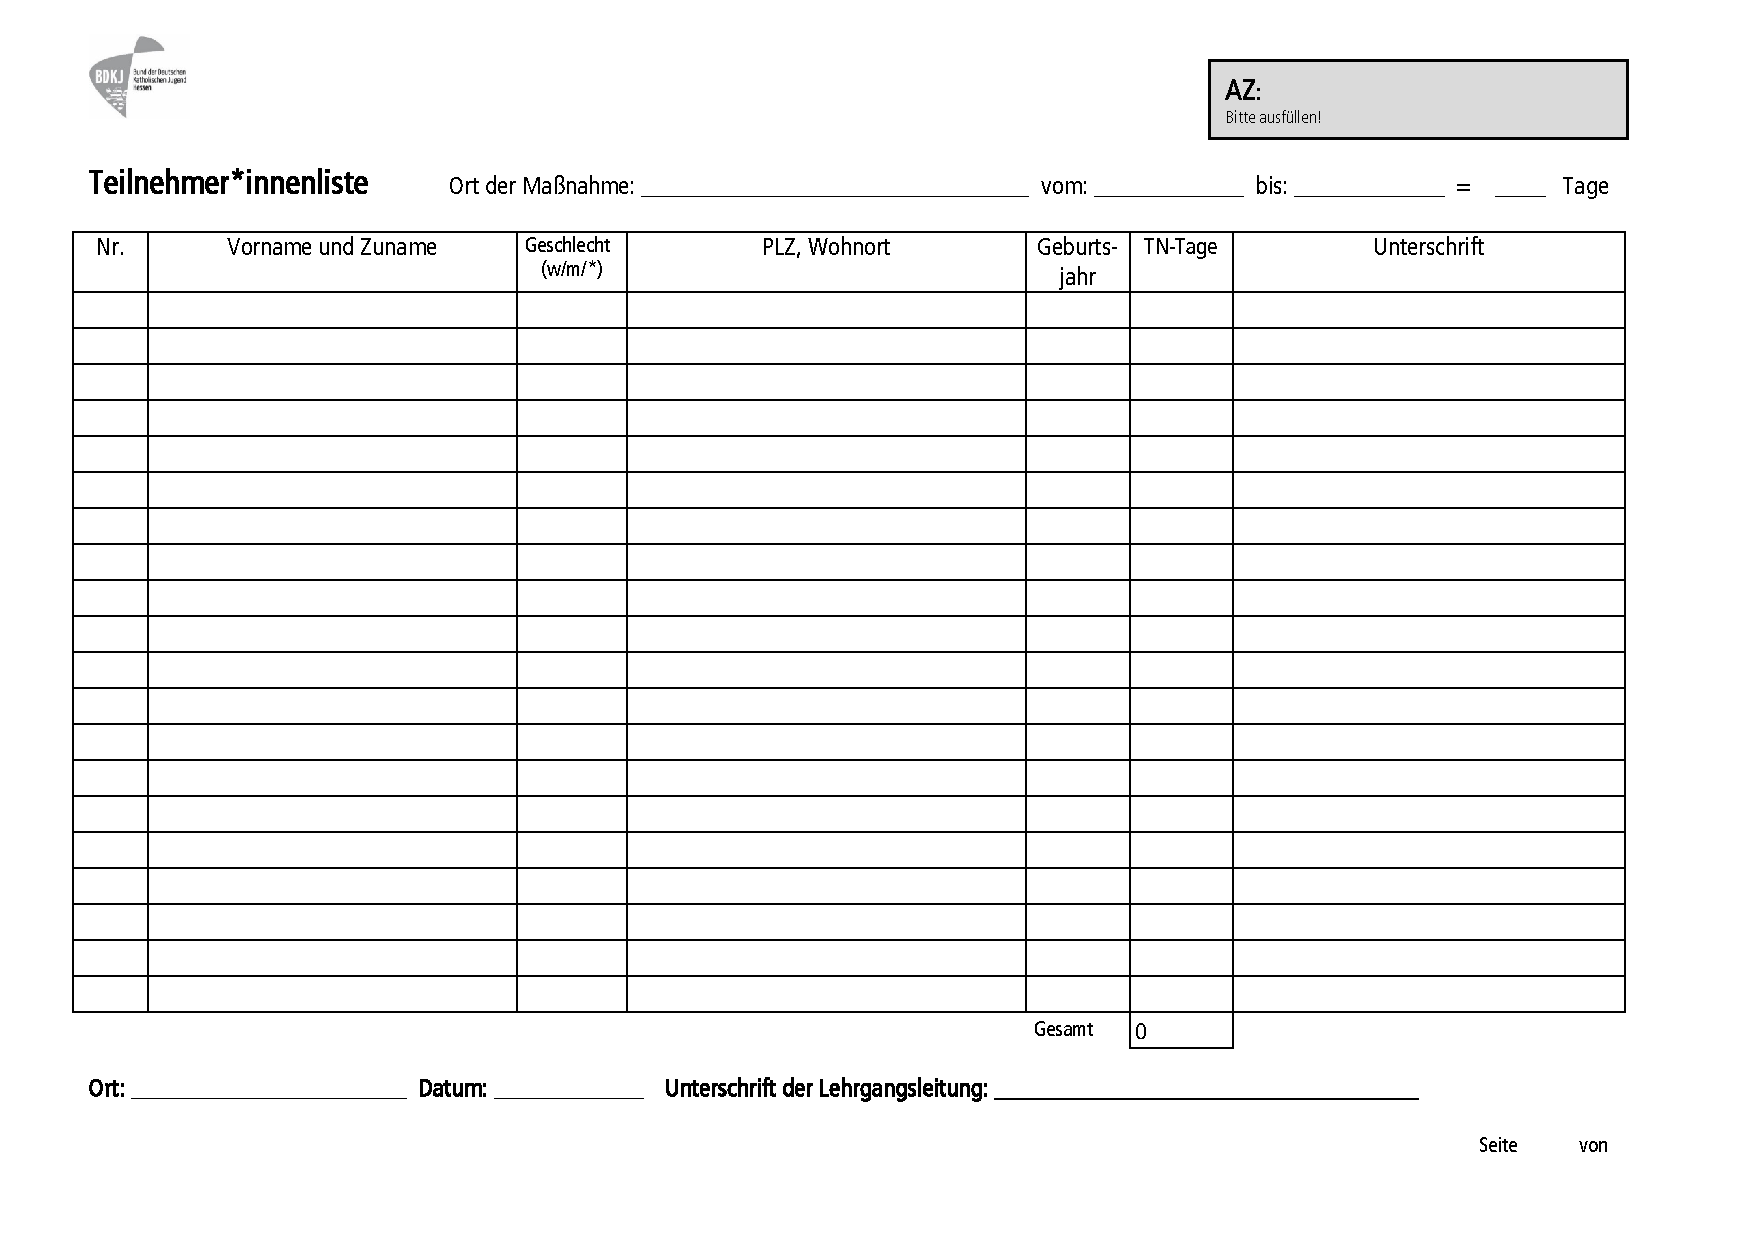
\includegraphics[width = \paperwidth, height = \paperheight] {bdkj-hesse.pdf}}}

\begin{document}
    \noindent \sffamily

    @foreach($members as $i => $chunk)
        \begin{tikzpicture}[remember picture,overlay,yscale=-1]
            \node[anchor=base west, text width=65.6mm] at (108.5mm,29.4mm) {\bfseries{\large{<<<!!$zipLocation!!>>>, <<<!!$countryName!!>>>}}};
            \node[anchor=base west, text width=25.4mm, align=center] at (185.0mm,29.4mm) {\bfseries{\large{<<<!!$dateFrom()!!>>>}}};
            \node[anchor=base west, text width=25.4mm, align=center] at (218.8mm,29.4mm) {\bfseries{\large{<<<!!$dateUntil()!!>>>}}};
            \node[anchor=base west, text width=8.5mm, align=center] at (253.0mm,29.4mm) {\bfseries{\large{<<<!!$durationDays!!>>>}}};

            @foreach($chunk as $j => $member)
                \node[anchor=base, text width=12.4mm, align=center] at ($(18.6mm, 50.0mm + 6.1mm * <<<$j%20>>>)$) {<<<$j+1>>>};
                \node[anchor=base, text width=62.2mm, align=center] at ($(56.2mm, 50.0mm + 6.1mm * <<<$j%20>>>)$) {<<<$memberName($member)>>>};
                \node[anchor=base, text width=18.5mm, align=center] at ($(96.85mm, 50.0mm + 6.1mm * <<<$j%20>>>)$) {<<<$memberGender($member)>>>};
                \node[anchor=base, text width=67.2mm, align=center] at ($(140.0mm, 50.0mm + 6.1mm * <<<$j%20>>>)$) {<<<$memberCity($member)>>>};
                \node[anchor=base, text width=17.2mm, align=center] at ($(182.5mm, 50.0mm + 6.1mm * <<<$j%20>>>)$) {<<<$memberBirthYear($member)>>>};
                \node[anchor=base, text width=17.2mm, align=center] at ($(199.6mm, 50.0mm + 6.1mm * <<<$j%20>>>)$) {<<<$durationDays>>>};
            @endforeach

            \node[anchor=base, text width=17.2mm, align=center] at ($(199.6mm, 50.0mm + 6.1mm * 20)$) {<<<$membersDays($chunk)>>>};

            \node[anchor=base west, text width=6.4mm, align=center] at (258.5mm,191.3mm) {<<<!!$i + 1!!>>>};
            \node[anchor=base west, text width=6.4mm, align=center] at (273.6mm,191.3mm) {<<<!!$pages!!>>>};

        \end{tikzpicture}

        \pagebreak
    @endforeach

\end{document}

